⑦ 次の図の制御系について以下の問いに答えよ.
\begin{figure}[H]
    \centering
    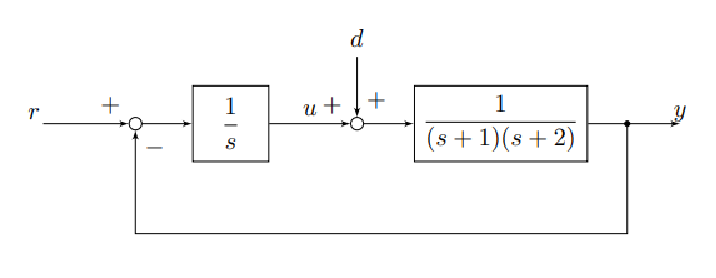
\includegraphics[scale=0.75]{figure1.pdf}
\end{figure}

a)\,$d(t)\equiv 0$としたときの目標値$r(t)$に対する定常位置偏差を求めよ.

b)\,$r(t)\equiv 0$であるとする.ランプ外乱$d(t)=t$を加えた時の$y(t)$の定常値を求めよ.

% a)\,定常速度偏差を求めるので,入力はランプ関数$r(t)=t$で,この関数のラプラス変換は$R(s)=\frac{1}{s^2}$である.

% ラプラス変換後の信号間の関係から,次の関係が得られる.
% $$
% E(s)=R(s)-P(s) K(s) E(s) \Rightarrow E(s)=\frac{1}{1+P(s) K(s)} R(s)
% $$
% これより,ラプラス変換の最終値の定理を用いて偏差の定常値を求める.
% $$
% \begin{aligned}
% E_s & =e(\infty)=\lim _{s \rightarrow 0} s E(s)=\lim _{s \rightarrow 0} s \frac{1}{1+\frac{1}{s(s+1)(s+2)}} \frac{1}{s^2}=\lim _{s \rightarrow 0} s \frac{s^3+3 s^2+2 s}{s^3+3 s^2+2 s+1} \frac{1}{s^2} \\
% & =\lim _{s \rightarrow 0} \frac{s^2+3 s+2}{s^3+3 s^2+2 s+1}=2
% \end{aligned}
% $$

% b)\,入力は恒常的に0,すなわち$r(t)=0$で,外乱としてステップ関数を考える.ステップ関数のラプラス変換は$R(s)=\frac{1}{s}$である.
% $$
% \begin{aligned}
% y(\infty) =\lim _{s \rightarrow 0} s Y(s)=\lim _{s \rightarrow 0} s \frac{\frac{1}{(s+1)(s+2)}}{1+\frac{1}{s(s+1)(s+2)}} \frac{1}{s}=\lim _{s \rightarrow 0} \frac{s}{s^3+3 s^2+2 s+1} = 0
% \end{aligned}
% $$